\documentclass{standalone}
\usepackage{amsmath}
\usepackage{amsfonts}
\usepackage{tikz}
\usetikzlibrary{arrows,shapes,positioning,shadows,trees}


\begin{document}
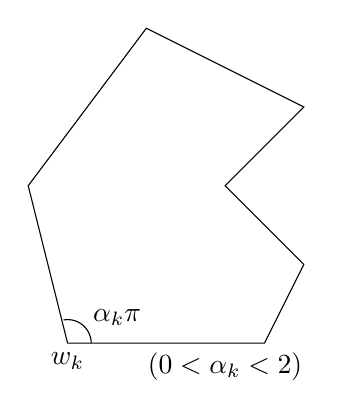
\begin{tikzpicture}
    \draw [-] (0,0) -- (2.5,0) -- (3,1) -- (2,2) -- (3,3) -- (1,4) -- (-0.5, 2) -- (0,0);
    % mark the angle (0,0) -- (2,5,0) and (0,0) -- (3,1)
    \draw (0.3,0) arc (0:100:0.3);
    % label as \alpha_k \pi
    \node[above right] at (0.2,0.1) {$\alpha_k \pi$};

    % label under (0,0) as w_k
    \node[below] at (0,0) {$w_k$};

    \node[below] at (2,0) {$(0<\alpha_k<2)$};
\end{tikzpicture}
\end{document}